\documentclass[a4paper,14pt]{extarticle}

% кодировка
\usepackage[utf8]{inputenc}
\usepackage[T2A]{fontenc}

% поля
\usepackage[left=30mm,right=15mm,top=20mm,bottom=20mm]{geometry}

% переносы слов
\usepackage[english,russian]{babel}

% шрифт Таймс
\usepackage{tempora}
\usepackage{newtxmath}

% межстрочный интервал
\usepackage[onehalfspacing]{setspace}

% интервал между абзацами (не регулируется ГОСТом)
\setlength{\parskip}{0.15em}

% отступ первой строки
\usepackage{indentfirst}
\setlength{\parindent}{1.25cm}

% скрытый структурный элемент
\newcommand{\hidedstructel}[1]{%
    \clearpage
    \phantomsection
    \section*{#1}%
}

% структурный элемент
\newcommand{\structel}[1]{%
    \hidedstructel{#1}
    \addcontentsline{toc}{section}{#1}%
}

% счетчик приложений
\usepackage{totcount}
\newtotcounter{annexcount}

% приложение
\renewcommand{\thesection}{\Asbuk{section}}
\newcommand{\annex}[1]{%
    \stepcounter{annexcount}%
    \clearpage
    \section{#1}%
}

% оформление структурного элемента и приложения
\usepackage{titlesec}
\titleformat{\section}
    [display]                   % форма
    {\filcenter\bfseries}       % формат полностью
    {ПРИЛОЖЕНИЕ \thesection}    % метка
    {0pt}                       % отступ от метки
    {}                          % код перед телом

% раздел
\newcommand{\sect}[1]{%
    \clearpage
    \setcounter{figure}{0}  % сбросить нумерацию внутри раздела
    \setcounter{table}{0}
    \setcounter{listing}{0}
    \subsection{#1}
    \renewcommand{\theparagraph}{\thesubsection.\arabic{paragraph}}
}
\titleformat{\subsection}{\filright\bfseries}{}{0pt}{\thesubsection\hspace{1em}}

% Переменная, которая регулирует отступы до и после заголовков подразделов. ГОСТ не регулирует этот вопрос
\newcommand{\headingsMargin}{0.5em}

\titlespacing*{\subsection}
    {\parindent}      % отступ слева
    {0pt}             % сверху
    {\headingsMargin} % снизу
\renewcommand{\thesubsection}{\arabic{subsection}}

% подраздел
\usepackage{placeins}
\newcommand{\subsect}[1]{%
    \FloatBarrier
    \subsubsection{#1}
    \renewcommand{\theparagraph}{\thesubsubsection.\arabic{paragraph}}
}
\titleformat{\subsubsection}{\filright\bfseries}{}{0pt}{\thesubsubsection\hspace{1em}}

\titlespacing*{\subsubsection}{\parindent}{\headingsMargin}{\headingsMargin}

% пункт
\newcommand{\parag}[1]{
    \paragraph{#1}
}
\titleformat{\paragraph}{\filright\bfseries}{\theparagraph}{1em}{ }  % для отступа
\titlespacing*{\paragraph}{\parindent}{\headingsMargin}{\headingsMargin}

% подпункт
\newcommand{\subparag}{
    \subparagraph{}
}
\titleformat{\subparagraph}[runin]{}{\thesubparagraph}{1em}{ }
\titlespacing*{\subparagraph}{\parindent}{0pt}{0pt}

% содержание
\usepackage{etoc}
\setcounter{tocdepth}{3}

% глубина нумерации разделов
\setcounter{secnumdepth}{5}

% перечисления
\usepackage{enumitem}
\setlist{
    topsep=0pt,                   % отступ сверху и снизу списка
    partopsep=0pt,                % то же самое
    leftmargin=0pt,               % отступ слева
    labelsep=0pt,                 % отступ метки
    align=left,                   % выравнивание метки
    listparindent = \parindent,   % отступ первой строки абзаца
    itemsep = \parskip,           % отступ между элементами
    parsep=0pt                    % отступ между абзацами и элементами
}
\setlist[itemize]{
    label=--~,  % в списках тире короткое, в тексте - длинное
    labelwidth=1.2em,
    itemindent=\parindent+\labelwidth
}
\setlist[enumerate]{
    label=\arabic*),
    labelwidth=1.4em,
    itemindent=\parindent+\labelwidth
}

% перечисление с буквенными метками
\AddEnumerateCounter*{\asbuk}{\c@asbuk}{7}
\newlist{asblist}{enumerate}{2}
\setlist[asblist]{
    label=\asbuk*),
    labelwidth=1.4em,
    itemindent=\parindent+\labelwidth
}

% подписи
\usepackage[singlelinecheck=false]{caption}
\DeclareCaptionLabelSeparator{gost}{~---~}
\captionsetup{labelsep=gost}

% иллюстрация
\newcommand{\fig}[3][1]{
    \begin{figure}[h]
        \centering
        \includegraphics[width=#1\textwidth]{#2}
        \caption{#3}\label{#2}
    \end{figure}
}
\renewcommand{\thefigure}{\thesubsection.\arabic{figure}}
\DeclareCaptionLabelFormat{gostfigure}{Рисунок #2}
\captionsetup[figure]{justification=centering, labelformat=gostfigure, position=bottom}
% font=singlespacing по умолчанию
%skip=-6pt

% листинг
\usepackage[newfloat, cache=false]{minted}
\newcommand{\lst}[2]{
    \begin{listing}[h]
        \centering
        \caption{#2}\label{#1}
        \begin{minipage}[t]{.8\textwidth}
            \inputminted[
                fontsize=\small,
                frame=single,
                breaklines,
                linenos
            ]{text}{#1}
        \end{minipage}
    \end{listing}
}
\renewcommand{\thelisting}{\thesubsection.\arabic{listing}}
\DeclareCaptionLabelFormat{custlisting}{Листинг #2}
\captionsetup[listing]{justification=raggedright, labelformat=custlisting, position=top}

% размер номера строки
\renewcommand{\theFancyVerbLine}{\rmfamily{\small \oldstylenums{\arabic{FancyVerbLine}}}}

% код в документе
\newenvironment{codepiece}[2]
{
    \VerbatimEnvironment
    \begin{listing}[h]
        \centering
        \caption{#2}\label{lst:#1}
        \begin{minipage}[t]{.8\textwidth}
            \begin{minted}[
                fontsize=\small,
                frame=single,
                breaklines,
                linenos
            ]{text}%
}{
            \end{minted}
        \end{minipage}
    \end{listing}
}

% таблица
\newenvironment{tbl}[3]
{
    \begin{table}[h]
        \small
        \centering
        \caption{#2}\label{tbl:#1}
        \begin{tabular}{|#3|}
            \hline
}{
            \hline
        \end{tabular}
    \end{table}
}
\renewcommand{\thetable}{\thesubsection.\arabic{table}}
\DeclareCaptionLabelFormat{gosttable}{Таблица #2}
\captionsetup[table]{justification=raggedright, labelformat=gosttable, position=top}

\usepackage{tabularx}

% объединение строк
\usepackage{multirow}
\newcommand{\mr}[2]{\multirow[t]{#1}{=}{#2}}

% колонки
\usepackage{array}
\newcolumntype{M}[1]{>{\centering\arraybackslash}m{#1}}
\newcolumntype{N}[1]{>{\raggedright\arraybackslash}p{#1}}

% заголовок таблицы
\usepackage{xparse}
\NewExpandableDocumentCommand\thead{t< t> O{1} m m}{%
    \IfBooleanTF{#1}{%
        \IfBooleanTF{#2}{%
            \multicolumn{#3}{|M{#4}|}{#5}%
        }{%
            \multicolumn{#3}{|M{#4}}{#5}%
        }
    }{%
        \IfBooleanTF{#2}{%
            \multicolumn{#3}{M{#4}|}{#5}%
        }{%
            \multicolumn{#3}{M{#4}}{#5}%
        }%
    }%
}

% код в таблице
\newenvironment{tabcode}[1]
{
    \VerbatimEnvironment
    \begin{minipage}[t]{#1\textwidth}
    \begin{minted}[fontsize=\small, breaklines]{text}
}{
    \end{minted}
    \end{minipage}
}

% длинная таблица
\usepackage{longtable}
\newenvironment{longtbl}[3]
{
    \small
    \begin{longtable}{|#3|}
        \caption{#2}\label{tbl:#1}\\
        \hline
}{
        \hline
    \end{longtable}
}

% математика
\usepackage{mathtools}  % amsmath
\numberwithin{equation}{subsection}

% графики
\usepackage{tikz, pgfplots}
\pgfplotsset{compat=newest}

\usepackage{adjustbox}
\usepackage{float}
\usepackage{url}

% источники
\usepackage[
    backend=biber,
    style=numeric-comp,
    bibstyle=gost-numeric,
    language = english,
    autolang = other,
    bibencoding=utf8,
    sorting = none,
]{biblatex}
\addbibresource{bibliography.bib}
\newcommand{\showbib}{%
    \structel{СПИСОК ИСПОЛЬЗОВАННЫХ ИСТОЧНИКОВ}%
    \printbibliography[heading=none]%
}

% отступы в источниках
\defbibenvironment{bibliography}
    {\list
        {}
        {\setlength{\leftmargin}{0pt}%
         \setlength{\itemindent}{\parindent}%
         \setlength{\itemsep}{0pt}%
         \setlength{\parsep}{0pt}}}
    {\endlist}
    {\item
     \printtext[labelnumberwidth]{%
        \printfield{labelprefix}%
        \printfield{labelnumber}%
     }%
     \hspace{0.5em}}

% метка без точки
\DeclareFieldFormat{labelnumberwidth}{#1}

% номер последней страницы
\usepackage{lastpage}

% счетчик источников
\newtotcounter{bibcount}
\AtEveryBibitem{
    \stepcounter{bibcount}%
}

% счетчики таблиц и рисунков
\usepackage{xassoccnt}
\newtotcounter{tblcount}
\DeclareAssociatedCounters{table}{tblcount}
\newtotcounter{figcount}
\DeclareAssociatedCounters{figure}{figcount}

% для отладки
%\usepackage{showframe}
%\renewcommand\ShowFrameLinethickness{0.25pt}
%\renewcommand*\ShowFrameColor{\color{red}}
%\usepackage{graphicx}


\usepackage{microtype}
\usepackage[extdef]{delimset}
\usepackage{csquotes} % иначе babel делает ворнинг
\usepackage{ragged2e}
\usepackage[hidelinks]{hyperref}
\usepackage{subfig}
\usepackage{tabularray}
\usepackage{epigraph}


\renewcommand{\div}{\operatorname{div}}


\begin{document}

\setcounter{page}{2}



\newcommand{\resultq}{0.7^{+0.3}_{-0.2}}
\newcommand{\resulti}{\brk!{55^{+5}_{-2}}\, {}^\circ}

\hidedstructel{АННОТАЦИЯ}

Исследуется симбиотическая двойная T Северной Короны. Предположительно, она является переменной звездой эллипсоидального типа, состоящей из красного гиганта и белого карлика.

% Считается, что она состоит из красного гиганта и белого карлика. Предполагая, что она является переменной эллипсоидального типа, мы симулируем кривые блеска и сравниваем их с наблюдениями в инфракрасных каналах $J$ и $K$.

Мы симулируем кривые блеска и сравниваем их с наблюдениями в инфракрасных каналах $J$ и $K$.
Мы решаем обратную задачу: определяем соотношение масс звезд-компаньонов и наклонение орбиты. Для этого используем байесовский подход и парадигму вероятностного программирования.

Мы получили, что $m_\text{giant} / m_\text{dwarf} = \resultq$, а наклонение орбиты равно $\resulti$, однако эти оценки смещаются в зависимости от выбора априорного распределения для соотношения масс.

Мы сравнили результаты при использовании спектра абсолютно черного тела и спектров, полученных с помощью модели звёздной атмосферы PHOENIX. Мы показали, что оценки параметров практически не меняются и чернотельная модель является хорошим приближением.

% Однако эти значения не фиксированные. Мы исследуем, как они смещаются в зависимости от выбора априорных распределений и модели звёздной атмосферы (чернотельной и PHOENIX).

Кривая блеска T Северной Короны имеет два минимума, и мы показали, что теория эллипсоидальной переменности недооценивает величину более глубокого из них. Это может означать, что требуется новая физическая модель для описания гравитационного потемнения в области красного гиганта, наиболее приближенной к белому карлику.


\begingroup

\parindent 0pt
\newlength{\pagewidth}\setlength{\pagewidth}{1.1em}

\newlength{\sectnum}\setlength{\sectnum}{8.4em}
\newlength{\ssectnum}\setlength{\ssectnum}{1em}
\newlength{\sssectnum}\setlength{\sssectnum}{2em}
\newlength{\paragnum}\setlength{\paragnum}{2.8em}

\newlength{\sssectindent}\setlength{\sssectindent}{2em}

\newcommand*{\entrybody}{%
    \raggedright%
    \etocname\nobreak%
    \leaders\etoctoclineleaders\hfill%
    \rlap{\makebox[\pagewidth][r]{\etocpage}}%
    \vspace{0.56em}% хак для отступа
}

\etocsetstyle{section}
    {}
    {\leavevmode\etocifnumbered{\leftskip \sectnum}{\leftskip 0pt}}
    {\normalsize\etocifnumbered%
        {\llap{\makebox[\sectnum][l]{ПРИЛОЖЕНИЕ \etocnumber}}%
            \parbox[t][][t]{\textwidth-\sectnum-\pagewidth}{\entrybody}}%
        {\parbox[t][][t]{\textwidth-\pagewidth}{\entrybody}}\par}
    {}
\etocsetstyle{subsection}
    {}
    {\leavevmode\leftskip \ssectnum}
    {\normalsize\llap{\makebox[\ssectnum][l]{\etocnumber}}%
        \parbox[t][][t]{\textwidth-\ssectnum-\pagewidth}{\entrybody}\par}
    {}
\etocsetstyle{subsubsection}
    {}
    {\leavevmode\setlength{\leftskip}{\sssectnum+\sssectindent}\relax}
    {\normalsize\llap{\makebox[\sssectnum][l]{\etocnumber}}%
        \parbox[t][][t]{\textwidth-\sssectnum-\pagewidth-\sssectindent}{\entrybody}\par}
    {}
\etocsetstyle{paragraph}
    {}
    {\leavevmode\setlength{\leftskip}{\paragnum+2\sssectindent}\relax}
    {\normalsize\llap{\makebox[\paragnum][l]{\etocnumber}}%
        \parbox[t][][t]{\textwidth-\paragnum-\pagewidth-2\sssectindent}{\entrybody}\par}
    {}

\etocsettocstyle{\hidedstructel{СОДЕРЖАНИЕ}}{}

\tableofcontents

\endgroup


\structel{ВВЕДЕНИЕ}

Симбиотические двойные — это системы, в спектре которых можно выделить линии поглощения, характерные для холодных звёзд, и эмиссионные линии, характерные для горячих туманностей.

Предполагается, что они состоят из близко расположенных красного гиганта и белого карлика, которые традиционно называются холодным и горячим компонентами. Из-за гравитации белого карлика красный гигант перестаёт быть сферически симметричным и приобретает каплевидную форму. Кроме того, может происходить перенос массы с красного гиганта на белый карлик, за счёт чего образуется аккреционный диск. Вещество может перетекать с помощью звёздного ветра --- или напрямую с поверхности, если холодный компонент полностью заполняет свою полость Роша.

Поскольку красный гигант не является сферически симметричным, при движении по орбите его блеск меняется. Такая переменность называется эллипсоидальной. Помимо чисто геометрического эффекта, на переменность также влияет гравитационное потемнение --- зависимость температуры от ускорения силы тяжести в конкретной точке поверхности звезды. Из-за него полюса красного гиганта будут наиболее горячими и яркими, а «носик», расположенный на экваторе и направленный в сторону точки Лагранжа --- наиболее холодным.

В данной работе анализируются кривые блеска T Северной Короны, измеренные в Крымской обсерватории ГАИШ МГУ в 1996--2003 и 2008-2021. На их основе мы определяем соотношение масс компонентов и наклонение орбиты — то есть решаем обратную задачу.

T Северной Короны --- повторная новая. Она вспыхивала в 1866, 1946 и, предполагается, должна вспыхнуть в 2024 \cite{OutburstAnnounce}. Повторные новые возникают, когда на поверхности белого карлика скапливается достаточно много водорода, перетекшего с красного гиганта, и начинается термоядерная реакция. Светимость в результате повышается на ${\sim} 10$ звёздных величин и медленно снижается в течение десятков дней.

Цель работы --- получить распределение вероятностей наклонения и соотношения масс компонентов двойной звезды T Северной Короны.

Методами исследования являются компьютерное моделирование кривых блеска и статистический вывод. Мы применили байесовский подход, воспользовавшись библиотекой для вероятностного программирования Turing.jl \cite{Turing}.

Вероятностное программирование --- парадигма программирования, предназначенная для работы с вероятностными моделями, которая позволяет автоматизировать статистический вывод и проверку гипотез. Главными идеями вероятностного программирования является автоматизированное применение теоремы Байеса, которое позволяет получить апостериорное распределение вероятностей для параметров задачи, и семплирование из него с помощью марковских цепей. Байесовский подход позволяет легко комбинировать данные от разнородных наблюдений.

Задачами работы являются:
\begin{enumerate}
    \item Численное моделирование физики переменности, получение модельных кривых блеска.
    \item Построение вероятностной модели, учитывающей статистические свойства экспериментальных данных.
    \item Получение апостериорного распределения вероятностей для параметров модели (наклонение, соотношение масс) и семплирование из него.
    \item Анализ распределения, получение оценок параметров и их доверительных интервалов.
\end{enumerate}

Настоящая работа была представлена на конференции МФТИ в 2024.

Новизна исследования заключается в применении байесовского подхода к обратной задаче астрофизики.

Значимость работы заключается в получении оценок параметров двойной звезды T Северной Короны и создании вероятностной модели переменности, учитывающей реалистичные модели звёздных атмосфер, которая может быть использована для анализа других симбиотических двойных.


\sect{Физика переменности}

Существует несколько типов переменных звёзд: затменные, пульсирующие и так далее. Считается, что T Северной Короны имеет \emph{эллипсоидальный} тип, т.е. в основе переменности лежит приливная деформация звезды.

В рамках эллипсоидальной модели \cite{Cherepashchuk} светимость в каждый момент времени определяется тремя эффектами: формой красного гиганта (мы предполагаем, что он заполняет свою полость Роша), гравитационным потемнением и потемнением к краю. В этой главе мы рассмотрим подробно каждый из трёх эффектов.

Белый карлик горячий и в основном излучает в ультрафиолете. Ультрафиолетовые наблюдения показывают, что затмения отсутствуют \cite{UV}. Мы исследуем данные в инфракрасном канале, поэтому вкладом белого карлика можно пренебречь.

Также мы пренебрегаем светимостью аккреционного диска и нагревом стороны красного гиганта, обращённой к белому карлику, за счёт излучения. В дальнейшем окажется, что модель недооценивает глубину одного из минимумов кривой блеска, и учет этих эффектов сделал бы ситуацию ещё хуже.
% Дело в том, что учёт обоих этих эффектов сделал бы минимум на кривой блеска менее глубоким

\subsect{Форма полости Роша}

На вещество массой $dm$, находящееся в двойной звёздной системе, действуют три силы: гравитация красного гиганта, гравитация белого карлика и центробежная сила. Область, в которой преобладает гравитация какого-либо из компонентов, называется его полостью Роша. Если вещество оказывается за пределами полости Роша, то оно перетекает на другую звезду или в космическое пространство.

Суммарный потенциал трёх сил равен
\begin{equation}
\Omega = 
-\frac{G m_\text{giant}}{r_1}
-\frac{G m_\text{dwarf}}{r_2}
-\frac{1}{2} (\omega \times r_3)^2
\label{eq:roche_generic}
\end{equation}
где $m_\text{giant}$ и $m_\text{dwarf}$ --- массы двух звёзд, $r_1$ --- расстояние до центра гиганта, $r_2$ --- расстояние до центра карлика, $r_3$ --- расстояние до центра масс, $\omega$ --- угловая скорость вращения звёзд по орбите.

Вещество красного гиганта, находясь под действием потенциала $\Omega$, заполняет некоторую эквипотенциальную поверхность, на которой $\Omega = \text{const}$. Одной из эквипотенциальных поверхностей является полость Роша. Она проходит через точку Лагранжа $L_1$, где все силы уравновешиваются и $\nabla \Omega = 0$.

В уравнении \eqref{eq:roche_generic} неявно предполагается, что гравитационный потенциал можно заменить потенциалом точечного тела. Это приближение оправданно, поскольку внешняя оболочка красных гигантов имеет очень низкую плотность, и масса в основном сосредоточена в практически сферическом ядре.

Найдём форму полости Роша численно. Для этого введём систему координат с центром в ядре красного гиганта, и направим ось $x$ в сторону карлика. Обозначим расстояние между центрами звёзд как $a$. Тогда \eqref{eq:roche_generic} примет вид
\[
\Omega =
-\frac{G m_\text{giant}}{\sqrt{x^2 + y^2 + z^2}}
-\frac{G m_\text{dwarf}}{\sqrt{(x - a)^2 + y^2 + z^2}}
-\frac{1}{2} \omega^2 \brk*{\brk*{x - a \frac{m_\text{dwarf}}{m_\text{giant} + m_\text{dwarf}}}^2 + y^2}
\]

Если обезразмерить координаты $(r \to r / a)$, обозначить соотношение масс $m_\text{giant} / m_\text{dwarf} = q$ и заметить, что в силу третьего закона Кеплера $\omega^2 = \dfrac{G}{a^3} \brk!{m_\text{giant} + m_\text{dwarf}}$, то получится
\begin{align*}
\Omega 
&= - \frac{G m_\text{giant}}{a} \brk[s]*{
    \frac{1}{r}
    + \frac{q^{-1}}{\sqrt{1 + r^2 - 2x}}
    + \frac{1 + q^{-1}}{2} \brk*{\brk*{x - \frac{1}{1+q}}^2 + y^2}
} \\
&= - \frac{G m_\text{giant}}{a} \brk[s]*{
    \frac{1}{r}
    + q^{-1} \brk*{
        \frac{1}{\sqrt{1 + r^2 - 2x}} - x
    }
    + \frac{1 + q^{-1}}{2} \brk!{x^2 + y^2}
    + \frac{q^{-1}}{1 + q}
}
\end{align*}

Последний член является константой и может быть отброшен. Таким образом, безразмерный потенциал равен
\begin{equation}
\Omega = \frac{1}{r} + q^{-1} \brk*{
    \frac{1}{\sqrt{1 + r^2 - 2x}} - x
}
+ \frac{1 + q^{-1}}{2} \brk!{x^2 + y^2}
\label{eq:roche_dekart}
\end{equation}
Или, в сферических координатах,
\begin{equation}
\Omega = \frac{1}{r} + q^{-1} \brk*{
    \frac{1}{\sqrt{1 + r^2 - 2r n_x}} - r n_x
}
+ \frac{1 + q^{-1}}{2} r^2 (1 - n_z^2)
\label{eq:roche_spherical}
\end{equation}
где введены направляющие косинусы $n_x = x / r$, $n_z = z / r$.

Уравнение \eqref{eq:roche_spherical} позволяет численно определить форму полости Роша. Для этого достаточно для всех направлений $(n_x, n_y, n_z)$ решить уравнение $\Omega(r) = \Omega_0.$

В качестве $\Omega_0$ необходимо взять значение потенциала в точке Лагранжа $L_1$. Её положение мы находим, решив уравнение $\dfrac{\partial \Omega(x, 0, 0)}{\partial x} = 0$.


\subsect{Гравитационное потемнение}

Гравитационное потемнение --- явление, при котором температура поверхности звезды зависит от ускорения силы тяжести в данной точке. Обычно его описывают формулой
\begin{equation}
T_\text{eff} \sim g^\beta
\label{eq:gravity_darkening}
\end{equation}

Величина $\beta$ зависит от типа внешней оболочки звезды. У голубых гигантов непосредственно под фотосферой находится зона лучистого переноса, и $\beta = 0.25$. У других звёзд, в том числе красных гигантов, внешней является зона конвекции, и $\beta$ принято считать равным $0.08$.

За счёт гравитационного потемнения звезда в симбиотической двойной системе излучает неравномерно (рис. \ref{pics/lemons.png}). Эффект также проявляется и у одиночных звёзд, если они вращаются быстро.

\fig{pics/lemons.png}{Пример распределения температур по поверхности холодного компаньона при $\beta = 0.08$ и $m_\text{giant} / m_\text{dwarf} = 1$.}

Отметим, что «носик» звезды лежит в точке Лагранжа, где $g = 0$. В соответствии с \eqref{eq:gravity_darkening}, эффективная температура в этой точке должна быть равна абсолютному нулю.

Мы закроем глаза на эту проблему и будем слепо применять \eqref{eq:gravity_darkening}, поскольку проблемная область не очень большая.

\parag{Закон фон Зейпеля}

Проще всего вывести \eqref{eq:gravity_darkening} для зоны лучистого переноса.

Давление внутри звезды складывается из давления газа и давления излучения: $P = P_g + \dfrac{4}{3} \dfrac{\sigma}{c} T^4$.
Градиент давления должен уравновешивать силу тяжести:
\[
\nabla P = \rho \vec g = -\rho \nabla \Omega
\]

Если рассмотреть смещение вдоль некоторого вектора $e$, то $d\Omega = (e \cdot \nabla \Omega)$,
\[
dP = -\rho d\Omega
\]

В частности, при $d\Omega = 0$ также $dP = 0$. Следовательно, $P$ постоянно на эквипотенциальных поверхностях и является функцией $\Omega$. Более того, $\rho = -\dfrac{dP(\Omega)}{d\Omega}$ тоже является функцией $\Omega$.

Вещество звезды должно подчиняться некоторому уравнению состояния:
\[
f(P, \rho, T) = 0
\]

Каким бы оно ни было, если $P = P(\Omega)$ и $\rho = \rho(\Omega)$, то и $T = T(\Omega)$. Поэтому эквипотенциальные поверхности также являются изобарическими, изопикническими и изотермическими.

Для лучистого переноса верно диффузное приближение: световой поток равен
\begin{equation}
F = -D \nabla U
\label{eq:Fick}
\end{equation}
где $U = \dfrac{4}{c} \sigma T^4$ --- плотность энергии, $D = \dfrac{1}{3} l c$ --- коэффициент диффузии, $l$ --- длина свободного пробега фотонов.

$U$ зависит только от температуры, которая является функцией $\Omega$. Следовательно,
\[
F = - D U'(T) T'(\Omega) \nabla \Omega
\]

$l$ и $D$ зависят от $\rho$, которая тоже является функцией $\Omega$. Поэтому на эквипотенциальных поверхностях
\[
F = \text{const} \cdot \nabla \Omega = \text{const} \cdot g
\]

В астрономии часто вводят эффективную температуру $T_\text{eff}$. По определению, это такая температура, что выполняется закон Стефана-Больцмана: 
\[
F = \sigma T_\text{eff}^4
\]
Обратите внимание на расхождение с формулой лучистого переноса \eqref{eq:Fick}. Если обычная температура на эквипотенциальных поверхностях является константой, то эффективная подчиняется
\[
T_\text{eff} \sim g^{1/4}
\]

Таким образом, в зоне лучистого переноса выполняется уравнение \eqref{eq:gravity_darkening} с $\beta = 1/4$.
Впервые этот результат был получен фон Зейпелем ровно 100 лет назад \cite{vonZeipel}.


\parag{Закон Люси}

В зоне конвекции, в отличие от зоны лучистого переноса, всё не так однозначно. Наиболее цитируемый результат был получен Львом Люси в 1967 году \cite{Lucy}:
\[
T_\text{eff} \sim g^{0.08}
\]

Люси рассмотрел случай, когда в зоне конвекции, начиная с некоторой небольшой глубины, удельная энтропия постоянна. Тогда температуру и плотность связывает уравнение адиабаты:
\begin{equation*}
T \rho^{1 - \gamma} = K
\label{eq:adiabat}
\end{equation*}
где $\gamma = 5/3$ --- показатель адиабаты, $K$ --- некоторая константа (константа адиабаты), характеризующая конкретную звезду.

Уравнение адиабаты можно переписать в виде
\begin{equation}
\log K = \log T + (1 - \gamma) \log \rho
\label{eq:adiabat_log}
\end{equation}

Люси предположил, что константа адиабаты зависит только от эффективной температуры и гравитации на поверхности:
\[
K(\log g, \log T_\text{eff}) = K_0
\]
Предположив $T \sim g^\beta$, можно получить
\[
\frac{\partial \log K}{\partial \log g}
+ \frac{\partial \log K}{\partial \log T_\text{eff}}
\underbrace{\frac{d \log T_\text{eff}}{d \log g}}_{\beta} = 0
\]
и выразить $\beta$ через частные производные:
\[
\beta = -\frac{\partial \log K / \partial \log g}{\partial \log K / \partial \log T_\text{eff}}
\]
Частные производные можно вычислить из \eqref{eq:adiabat_log}. Люси использовал для этого таблицы конвективных моделей звёзд из книги Бейкера (1963). Он получил, что $\beta$ слабо зависит как от соотношения между водородом и гелием, так и от соотношения между длиной смешивания и высотой однородной атмосферы. Для практических применений Люси предлагает использовать
\[
\beta \approx 0.08
\]
Именно это значение используется в настоящей работе.


\parag{Коэффициент Кларета}

Полученные выше законы $T_\text{eff} \sim g^{1/4}$ и $T_\text{eff} \sim g^{0.08}$ относятся к болометрической светимости.
Но наблюдения, как правило, производятся в некоторой узкой полосе длин волн, причем спектр реальных звёзд далек от чернотельного.

Поэтому Антоний Кларет предлагает \cite{ClaretGravity} ввести коэффициент $y(\lambda)$, по определению равный
\begin{equation}
y(\lambda)
\coloneq \brk*{
    \frac{\partial \ln I(\lambda)}{\partial \ln g}
}_{T_\text{eff}}
+\brk*{
    \frac{\partial \ln I(\lambda)}{\partial \ln T_\text{eff}}
}_g
\brk3{
    \underbrace{
        \frac{d \ln T_\text{eff}}{d \ln g}
    }_{\beta}
}
\label{eq:ClaretGravity}
\end{equation}
где $I(\lambda)$ --- интенсивность излучения в полосе $\lambda$.

Кларет вычислил $y(\lambda)$ численно, используя модели ATLAS и PHOENIX. Оказалось, что $y(\lambda)$ зависит от эффективной температуры, гравитации и скорости микротурбулентности.

На рис. \ref{fig:ClaretGravity} показаны примеры полученных им зависимостей для инфракрасных фильтров $J$ и $K$.

\begin{figure}[h]
\centering
\subfloat{
    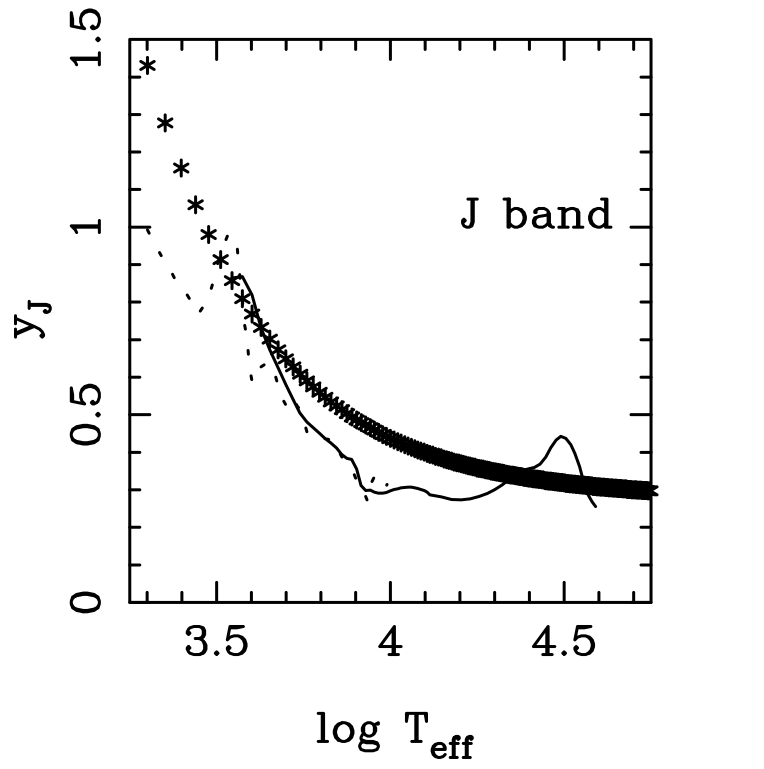
\includegraphics[height=0.4\textwidth]{pics/Claret GDC J.png}
}
\subfloat{
    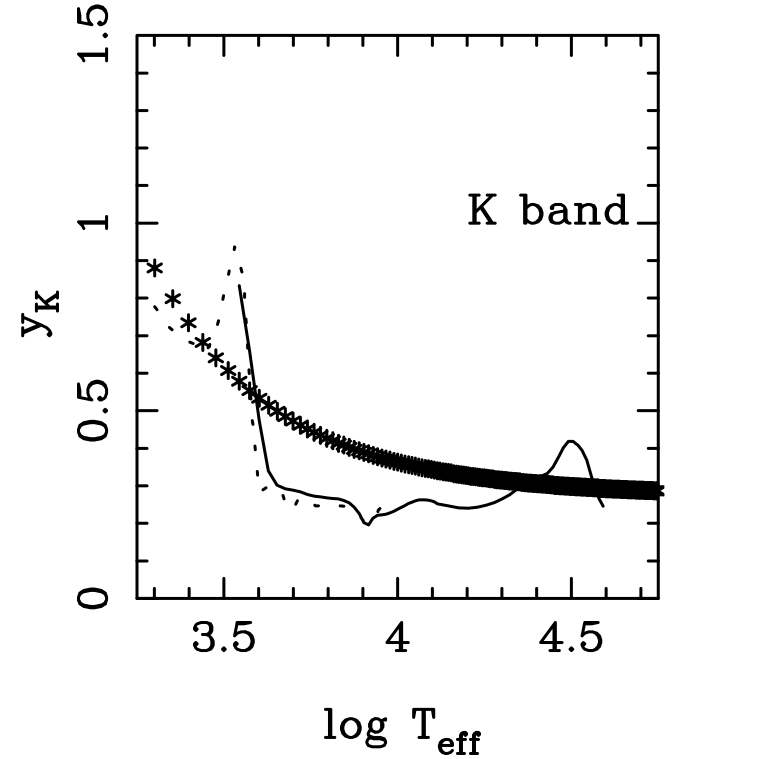
\includegraphics[height=0.4\textwidth]{pics/Claret GDC K.png}
}
\caption{Коэффициент гравитационного потемнения \eqref{eq:ClaretGravity} для фильтров $J$ и $K$ в зависимости от эффективной температуры.
Звёздочками обозначена модель абсолютно черного тела, сплошной линией --- модель ATLAS, пунктирной --- PHOENIX. Параметры моделей: $\log g = 4$ см/с+2, $v_\text{mic} = 2$ км/с, металличность $\log [\text{M}/\text{H}] = 0$.
Изображения взяты из \cite{ClaretGravity}.}
\label{fig:ClaretGravity}
\end{figure}

Данный подход, хоть и является более правильным, не очень полезен для настоящей работы. Он позволяет вычислить производную интенсивности по гравитации при определенной температуре, но не позволяет напрямую получить распределение температур по поверхности звезды. Поэтому мы будем использовать простой закон $T_\text{eff} \sim g^{0.08}$.


\parag{Модель Лары-Рьётора}

Самую новую модель на сегодняшний день предложили в 2012 году Франческо Лара и Мишель Рьётор \cite{LaraRieutord}. Они приняли приближение, что поток излучения всегда антипараллелен гравитации:
\[
\vec F = -f(r, \theta, \varphi) \vec g
\]
где $f$ --- некоторая положительная функция, которую нужно найти.

В установившемся режиме всюду, кроме центра звезды, поток энергии должен сохраняться:
\[
\div F = 0
\]
Следовательно,
\[
\vec g \cdot \nabla f + f \nabla \cdot \vec g = 0
\]
Если ввести $\vec n = -\vec g / g$, то
\[
\vec n \cdot \nabla \log f = \frac{\nabla \cdot \vec g}{g}
\]
Решение можно получить, проинтегрировав это уравнение вдоль \emph{линии поля} --- кривой, которая в каждой точке касается вектора $\vec n$. Рассмотрим линию поля, которая начинается в точке $O$ (гравитационном центре звезды) и заканчивается в некоторой точке $A$. Тогда
\begin{equation*}
f(A) = f_0 \exp \left(
    {}\int\limits_O^A \frac{\nabla \cdot \vec g}{g} ds
\right)
\label{eq:LaraSolution}
\end{equation*}
где $f_0$ --- нормировочная константа, определяющаяся полной светимостью звезды.

Интеграл можно вычислить численно, выразив $g = \nabla \Omega$ с помощью формулы для потенциала Роша \eqref{eq:roche_spherical}.

Как показали Лара и Рьётор, в результате снова приблизительно получится степенной закон $T_\text{eff} \sim g^\beta$.

Величина $\beta$ зависит от соотношения масс компаньонов и процента заполнения полости Роша, авторы приводят соответствующие таблицы. Для большинства случаев $\beta$ лежит в интервале 0.20--0.25.

В пределе нулевого заполнения полости Роша, когда приливной деформацией можно пренебречь, $\beta \to 0.25$, что соответствует закону фон Зейпеля.

Несмотря на красоту модели Лары-Рьётора, в данной работе мы используем общепринятый закон Люси с $\beta = 0.08$, чтобы иметь возможность сравнивать наши результаты с другими работами по T Северной Короны.


\subsect{Потемнение к краю}

Звёзды не являются ламбертовскими источниками. Дело в том, что наблюдатель получает излучение с внешних слоев звезды вплоть до оптической глубины $\tau \approx 1$. Если наблюдение происходит перпендикулярно поверхности, то «просвечивают» более глубокие слои фотосферы, чем при наблюдении под углом \cite{StellarSpectroscopy}.

Как правило, глубокие слои фотосферы являются более горячими. Соответственно, края звезды, поскольку наблюдаются под углом, кажутся более красными и тёмными, чем её центр.

% Они имеют атмосферу ненулевой толщины, и, когда мы смотрим на поверхность под углом, свет проходит в атмосфере больший путь. Поэтому края звёзд кажутся более красными и тёмными, чем их центр.

Потемнение к краю определяется численно, с использованием моделей ATLAS \cite{AtlasDarkening} и PHOENIX \cite{PHOENIX}. Антоний Кларет показал, что его можно профитировать формулой
\begin{equation}
I = I_0 \cdot \brk2{
    1 - a_1 \brk!{1 - \mu^{1/2}} - a_2 \brk!{1 - \mu} - a_3 \brk!{1 - \mu^{3/2}} - a_4 \brk!{1 - \mu^2}
}
\label{eq:ClaretDarkening}
\end{equation}
где $\mu = (\vec n \cdot \vec d)$ --- косинус угла между лучом зрения и нормалью к поверхности. Коэффициенты $a_i$ зависят от температуры, металличности и ускорения силы тяжести, Кларет приводит соответствующие таблицы \cite{ClaretDarkening}.

Температура и ускорение силы тяжести варьируются по поверхности звезды. Чтобы это учесть, мы интерполируем коэффициенты из таблиц.

В данной работе интерполяция осуществляется только по температуре. Зависимость от силы тяжести более слабая, и мы приняли, что на всей поверхности звезды $\log g = 4$ см/с+2.


\sect{Вычисление синтетических кривых блеска}

Чтобы сопоставлять экспериментальные значения с теоретическими, необходимо вычислять синтетические кривые блеска.


Яркость звезды определяется интегралом:
\begin{equation}
L = \int\limits_{\mu > 0}
dS \cdot
I_\perp (\theta, \varphi) \cdot \mu \cdot
\operatorname{LimbDarkening}(\mu)
\label{eq:flux_integral}
\end{equation}
где $\mu = (\vec n \cdot \vec d)$ --- косинус угла между нормалью к поверхности и направлением на наблюдателя, $I_\perp(\theta, \varphi)$ --- интенсивность излучения данной точки звезды в данном спектральном канале при $\mu = 1$, $\operatorname{LimbDarkening}(\mu)$ --- функция потемнения к краю. Интегрирование производится по видимой части поверхности, где $\mu > 0$.

Чтобы получить кривую блеска, нужно вычислить интеграл \ref{eq:flux_integral} для разных фаз (и, соответственно, разных направлений на наблюдателя).

Это происходит следующим образом:
\begin{enumerate}
    \item Вычисление формы звезды (полости Роша). Для этого мы сначала создаём сферическую сетку, а затем деформируем её так, чтобы результирующая поверхность оказалась эквипотенциальной для потенциала \eqref{eq:roche_spherical}.
    \item Вычисление ускорения силы тяжести и температуры в каждой вершине. Ускорение силы тяжести мы получаем, вычисляя $\nabla \Omega$ автоматическим дифференцированием с помощью дуальных чисел. Температуру мы вычисляем, используя закон Люси $T_\text{eff} = T_0 \brk2{\frac{g}{g_0}}^{0.08}$. В качестве $g_0$ и $T_0$ мы берем значения на экваторе звезды в точке, наиболее удаленной от «носика».
    \item Вычисление $I_\perp$ в каждой вершине. Мы используем спектры из модели звёздных атмосфер PHOENIX и сворачиваем их с полосой пропускания фильтра.
    \item Вычисление нормалей и коэффициентов потемнения к краю $a_i(T)$ для каждой грани.
    \item Суммирование по видимым граням с учетом потемнения к краю и преобразование к звёздной величине по формуле $m = -2.5 \log_{10} L$.
\end{enumerate}

Блеск вычисляется в условных единицах. Это позволяет не учитывать реальные размеры звезды и ослабление излучения с расстоянием. Но в результате при логарифмировании появится смещение на некоторую подгоночную константу.

Остановимся подробнее на некоторых оптимизациях и деталях реализации.

\subsect{Полигональная сетка}

Чтобы проинтегрировать поток излучения по поверхности звезды, мы разбиваем её на треугольники. Желательно расположить точки более-менее равномерно по поверхности звезды, тогда треугольников понадобится меньше.

Для этого мы используем алгоритм Катмулла-Кларка из библиотеки Meshes.jl, который итеративно разбивает грани на более маленькие (рис. \ref{pics/Catmull-Clark.png}). Он часто применяется в компьютерной графике для создания гладких поверхностей.

\fig[0.6]{pics/Catmull-Clark.png}{Алгоритм Катмулла-Кларка, итерации с нулевой по третью. Мы используем 4 итерации, что даёт хороший баланс между точностью и количеством вершин.}

Этот алгоритм создаёт сетку из четырёхугольников, близкую к сферической. У четырёхугольников не всегда можно определить нормаль, поэтому мы дополнительно разбиваем каждый четырёхугольник на два треугольника.

Затем мы деформируем сферическую сетку, домножая радиус-вектор $\vec n$ каждой вершины на число $r$ такое, что $\Omega(r \vec n) = \text{const}$, где $\Omega$ --- потенциал Роша \eqref{eq:roche_spherical}.

Форма звезды определяется соотношением масс звёзд $q$ и коэффициентом заполнения полости Роша $\rho.$ Мы предполагаем, что $\rho = 1$, потому что это упрощает задачу и потому что при $\rho < 1$ амплитуда переменности быстро уменьшается.

Впоследствии нам понадобится дифференцировать блеск по $q$. Но создание сетки включает в себя численное решение уравнения. Это итеративный процесс, который сложно дифференцировать. Поэтому мы заранее вычисляем сетку для набора значений $q$, сохраняем для каждой вершины интерполяционный полином $r(q)$ и дифференцируем уже его.

С изменением $q$ сильно меняется размер полости Роша (если зафиксировано расстояние между компаньонами) и, соответственно, общая яркость звезды. Это нежелательно для семплирования, поскольку делает параметры $q$ и $\text{offset}$ (см. таблицу \ref{tab:model}) сильно скоррелированными. Поэтому мы дополнительно нормируем радиус-векторы вершин сетки на радиус-вектор вершины, наиболее удалённой от «носика» звезды.

Примеры синтетических кривых блеска для разных соотношений масс приведены на рис. \ref{pics/curves.pdf}.

\fig[0.8]{pics/curves.pdf}{Примеры синтетических кривых блеска для разного соотношения масс. Первому (глубокому) минимуму соответствует наблюдение со стороны «носика» --- наиболее холодной части звезды. Второму минимуму соответствует наблюдение с противоположной «носику» стороны. Максимумам соответствует наблюдение с боковых сторон, тогда достигается наибольшая видимая площадь.}













\sect{Данные}

\subsect{Блеск}\label{sect:Brilliance}

Мы используем данные о блеске T Северной Короны, полученные в Крымской обсерватории ГАИШ МГУ.

Измерения проводились в 152 ночи, разбросанные по интервалам суммарной продолжительностью 20 лет (1996--2003 и 2008--2021 годы). Данные охватывают порядка тридцати 227-суточных периодов, но с малым количеством точек на период.

В некоторые ночи измерения проводились повторно (естественно, с разными результатами). Мы оставили эти измерения такими, какие они есть, поскольку это не препятствует применению нашей вероятностной модели.

Измерения проводились в инфракрасных фильтрах $J$ ($\lambda = 1.25,\ \Delta \lambda = 0.33$ мкм) и $K$ ($\lambda = 2.2,\ \Delta \lambda = 0.4$ мкм). Общее число точек по каждому из каналов составило 209.

\fig[0.75]{pics/raw.pdf}{Измерения блеска T Северной Короны}

Чтобы определить погрешность, наблюдатели одновременно с T Северной Короны измеряли некую референсную звезду, чья звёздная величина предполагалась постоянной. Полученная таким способом погрешность иногда оказывалась нулевой, поскольку звёздная величина измерялась с точностью до двух знаков после запятой и иногда наблюдалось полное совпадение.

Из рис. \ref{pics/raw.pdf} видно, что разброс точек заметно больше, чем фотометрические ошибки.
Поэтому мы добавили ко всем измерениям некоторую общую погрешность:
\[
\tilde \sigma_t = \sqrt{\sigma_t^2 + \sigma_\text{common}^2}
\]

Добавочная погрешность символизирует все источники ошибок, не являющиеся погрешностью прибора. Это могут быть, например, быстрые изменения блеска звезды, вызванные тёмными пятнами.

Поскольку точная физическая природа $\sigma_\text{common}$ неизвестна, мы сделали её случайным параметром, который подбирается в процессе семплирования.

Ценой такого подхода является то, что мы не можем использовать некоторые статистические критерии, такие как $\chi^2$, чтобы оценить согласие модели с данными. Семплер подберёт достаточно большую величину погрешности, чтобы правдоподобие было высоким, тогда $\chi^2$ автоматически будет близко к 1. Но это не будет означать, что модель хорошо описывает данные.

Вместо критерия $\chi^2$ мы будем использовать runs test. Этот статистический критерий опирается не на величину отклонений данных от модели, а на последовательность их знаков, что позволяет оценить согласие модели с данными без информации о погрешности.


\subsect{Лучевые скорости}

Лучевой скоростью называется проекция скорости на луч зрения. Её можно измерить, наблюдая за смещением спектральных линий, вызванным эффектом Доплера.

В течение периода лучевая скорость меняется и соответственно меняется смещение спектральных линий. Можно нанести смещения на график и оценить амплитуду лучевой скорости.

Если проводить измерения в инфракрасном диапазоне, то полученная скорость будет относиться к холодному красному гиганту. Если же проводить измерения эмиссионной линии H$\alpha$, то полученная скорость будет относиться к аккреционному диску вокруг белого карлика \cite{H_alpha}.

\fig[0.5]{pics/radial-velocities.png}{Лучевые скорости холодного компонента T Северной Короны, измеренные в разных обсерваториях. Изображение взято из \cite{RadialVelocities}.}

Лучевые скорости красного гиганта известны точнее, поскольку были независимо измерены разными обсерваториями. В метаанализе Fekel et al. \cite{RadialVelocities} на их основе показано, что орбита T Северной Короны является круговой, а период равен $227.5687 \pm 0.0099$ суток.

\parag{Ограничение, вытекающее из предела Чандрасекара}\label{sect:Chandrasekhar}

Зная лучевую скорость и период красного гиганта, с помощью предела Чандрасекара можно ограничить возможные соотношения масс компонентов и наклонения орбиты. Покажем, как это сделать.

В работе Fekel et al. \cite{RadialVelocities} показано, что проекция радиуса орбиты холодного компонента T Северной Короны на луч зрения равна:
\[
a_\| \coloneq a_\text{giant} \cdot \sin i = (74.77 \pm 0.53) \cdot 10^6 \text{ км}
\]
%
%Зная $a_\|$, мы можем ограничить возможные наклонения орбиты $i$ и соотношения масс.
%
Радиусы орбит компонентов обратно пропорциональны их массам. Обозначим
\[
\frac{a_\text{dwarf}}{a_\text{giant}} = \frac{m_\text{giant}}{m_\text{dwarf}} = q
\]
Запишем третий закон Кеплера:
\[
P^2 = \frac{4\pi^2}{G} \frac{\brk!{a_\text{dwarf} + a_\text{giant}}^3}{m_\text{dwarf} + m_\text{giant}}
= \frac{4\pi^2}{G} \frac{a_\text{giant}^3}{m_\text{dwarf}} \frac{(1 + q)^3}{(1 + q)}
= \frac{4\pi^2}{G} \frac{a_\|^3}{m_\text{dwarf}} \frac{(1 + q)^2}{\sin^3 i}
\]
Получается следующая зависимость между $q$ и наклонением орбиты $i$:
\[
\sin^3 i = \frac{4\pi^2}{G} \frac{a_\|^3}{P^2 m_\text{dwarf}} (1 + q)^2
\]

% Масса белого карлика не может быть больше предела Чандрасекара. Следовательно,
% \[
% i > \arcsin \sqrt[3]{
%     \frac{4\pi^2}{G} \frac{a_\|^3}{1.44 M_\odot T^2} (1 + q)^2
% }
% \]

Масса белого карлика не может быть больше предела Чандрасекара. Если подставить числовые значения для T Северной Короны, то это даёт следующее ограничение на $i$ и $q$:
\[
\sin^3 i > 0.224 \cdot (1 + q)^2
\]
Разрешённая область изображена на рис. \ref{pics/sine.pdf}:

\fig[0.45]{pics/sine.pdf}{Допустимые значения наклонения орбиты и соотношения масс компонентов T Северной короны в соответствии с пределом Чандрасекара и наблюдениями лучевых скоростей холодного компонента.}


% \subsect{Период}

% Определение периода --- нетривиальная задача.

% Первое, что приходит в голову, --- это применить дискретное преобразование Фурье. Но, поскольку промежутки между измерениями не одинаковые, это невозможно.

% Чаще всего в астрономии строят периодограмму Ломба-Скаргла. Для этого для большого количества различных частот производится фитирование формулой
% \[
% f(t) = a \sin(\omega t) + b \cos(\omega t) + c
% \]
% и вычисляется «мощность», которая показывает, насколько хорошим получилось фитирование. Поскольку для метода наименьших квадратов существуют готовые формулы, большое число частот можно обработать за разумное время.

% \fig{pics/periodogram.pdf}{Периодограмма Ломба-Скаргла для измерений блеска T Северной Короны в спектральном канале $K$. Максимум мощности соответствует периоду 113.75 суток.}

% Недостатком является то, что периодограмма Ломба-Скаргла предполагает синусоидальную зависимость, в то время как из рис. \ref{pics/curves.pdf} видно, что модельные кривые блеска не являются синусоидами, поскольку минимумы имеют разную глубину.

% В результате, если слепо применить периодограмму Ломба-Скаргла (рис. \ref{pics/periodogram.pdf}), то получится неверный период 113.75 суток.

% Чтобы получить правильную картинку с двумя минимумами (рис. \ref{pics/raw.pdf}), мы домножили период на 2 и получили 227.5 суток. Это согласуется с работой \cite{RadialVelocities}, в которой на основе измерений лучевых скоростей период был оценен как $227.5687 \pm 0.0099$ суток.

% Следует отметить, что период может меняться со временем. Момент импульса двойной системы должен сохраняться, но, поскольку звёзды обмениваются массой, может изменяться суммарный момент инерции и соответственно угловая скорость. Поэтому бессмысленно пытаться вычислить период с высокой точностью.


\subsect{Температура}\label{sect:temperature}

У звёзд, как правило, нет определённой температуры, поскольку она, как минимум, варьируется с глубиной в толще фотосферы. Чтобы охарактеризовать излучение звезды как целого, вводят эффективную температуру, которая по определению равна
\begin{equation}
T_\text{eff} = \brk*{\frac{L}{\sigma S}}^{1/4}
\label{eq:Teff}
\end{equation}
где $L$ --- светимость звезды, $S$ --- её площадь, $\sigma$ --- постоянная Стефана-Больцмана.

Эффективная температура --- это одно число. Именно ей параметризуют модели звёздных атмосфер ATLAS \cite{AtlasSpectra, AtlasDarkening} и PHOENIX \cite{PHOENIX}.

Аналогично, чтобы охарактеризовать излучение участка звезды, можно ввести локальную эффективную температуру:
\begin{equation}
T_\text{local eff} = \brk*{\frac{F}{\sigma}}^{1/4}
\label{eq:Tlocaleff}
\end{equation}
где $F$ --- плотность потока излучения от данного участка.

% Локальную эффективную температуру можно воспринимать как физическую температуру, некоторым образом усреднённую по глубине, но не по поверхности фотосферы.

Если звезда сферически симметричная, то $T_\text{eff} = T_\text{local eff}$.

В нашем случае это не так: звезда приливно деформирована, локальная эффективная температура зависит от координаты и предположительно определяется законом Люси:
\begin{equation}
T_\text{local eff} = T_0 \brk*{\frac{g}{g_0}}^{0.08}
\label{eq:Lucy}
\end{equation}
где $T_0$ и $g_0$ --- локальная эффективная температура и ускорение силы тяжести в какой-то выбранной точке.

Нам необходимо знать константу $T_0$: это позволит строить карты температур и получать синтетические кривые блеска.

В качестве данных у нас есть две оценки эффективной температуры (3400 ${}^\circ$K и 3600 ${}^\circ$K), сделанные разными способами на основе спектра, снятого 6 июня 2004 года \cite{TCRBtemperature}.

Эти оценки представляют собой локальную эффективную температуру \eqref{eq:Lucy}, некоторым образом усреднённую по части поверхности звезды, видимой в тот день.

Разброс оценок (200 ${}^\circ$K) сопоставим с разбросом локальных эффективных температур по поверхности звезды (рис. \ref{pics/lemons.png}).

Мы выбрали в качестве $T_0$ середину диапазона --- $3500\ {}^\circ K$ --- и присвоили её точке, наиболее удалённой от «носика». Эта точка не является ни самой горячей, ни самой холодной, поэтому она должна с достаточной точностью представлять среднюю температуру.

Теоретически можно было бы выбрать $T_0$ случайным параметром и подбирать его в процессе семплирования. Можно было пытаться добиться того, чтобы проинтегрированный по поверхности модельный спектр имел линии той же эквивалентной ширины / имел то же соотношение $J-K$, что и измеренный. Но мы решили, что это неоправданно усложнит модель, не дав ей выигрыша в точности.

Рассмотрим теперь, как в работе \cite{TCRBtemperature} была получена температура.

% Теоретически можно было бы вычислить фазу, в которой была видна звезда, и подобрать $T_0$ такое, чтобы проинтегрированный по поверхности модельный спектр имел линии той же эквивалентной ширины / имел то же соотношение $J-K$, что и измеренный.



\parag{Спектрометрический метод}

\setlength{\epigraphrule}{0pt}
\epigraph{\emph{A picture may be worth a thousand words, but a spectrum is worth a thousand pictures.}}

В спектрометрическом методе вычисляется эквивалентная ширина линий
\[
W_\lambda \coloneq \int \brk*{1 - \frac{F}{F_0}} d \lambda
\]
где $F_0(\lambda)$ --- предполагаемый световой поток на данной длине волны в отсутствие линии.

Эквивалентная ширина зависит от столбцовой плотности поглощающих частиц $\rho$, силы осциллятора $f$ (величины, отражающей вероятность перехода между уровнями энергии), заселённости начального уровня $n$ и его статистического веса $g$:
\begin{equation}
W_\lambda = W_\lambda(n(T) \rho g f)
\label{eq:W}
\end{equation}

Эта зависимость называется \emph{кривой роста} \cite{StellarSpectroscopy}. Она состоит из нескольких сегментов: линейного (для слабых линий), пологого $\brk!{W_\lambda \sim \sqrt{\ln x}}$ и сегмента затухания $\brk!{W_\lambda \sim \sqrt{x}}$.

Столбцовая плотность $\rho$ зависит от относительного содержания химического элемента, например [Fe/H].

Заселённость $n(T)$ определяется в два этапа: сначала с помощью формулы Саха вычисляется доля атомов в нужной степени ионизации, затем с помощью распределения Больцмана вычисляется доля атомов на нужном уровне энергии. 

Зависимость $n(T)$ определяется энергией уровней. Поэтому разные линии одного элемента по-разному отвечают на изменение температуры.

Сила осциллятора и статистический вес --- табличные величины, в работе \cite{TCRBtemperature} они взяты из VALD (Vienna Atomic Line Database).

На практике \eqref{eq:W} вычисляется с помощью атмосферных моделей, таких как PHOENIX:
\begin{equation}
W_\lambda = \operatorname{PHOENIX}(T_\text{eff}, \log g, \text{[Fe/H]})
\label{eq:W_PHOENIX}
\end{equation}

С помощью атмосферных моделей можно вычислять относительное содержание элемента по эквивалентной ширине линии и эффективной температуре.

В работе \cite{TCRBtemperature} авторы подбирают $T_\text{eff}$ такую, что относительное содержание, вычисленное для разных линий одного элемента (железа), оказывается одинаковым.

Они получают 3600 ${}^\circ$K.


\parag{Фотометрический метод}

В фотометрическом методе вычисляется показатель цвета --- разность звёздных величин в фильтрах $J$ и $K$ (или других).

Для T Северной Короны $J - K$ слабо меняется с фазой и приблизительно равно 1.19.

Примечательно, что в $\text{ваттах}/\text{м}^2$ блеск в фильтре $J$ больше блеска в фильтре $K$, поэтому разность звёздных величин $m_J - m_K$ должна быть отрицательной. Но она положительная, поскольку нуль звёздной величины зависит от фильтра. По соглашению, он соответствует блеску Веги в данном фильтре.

Далее вычисленное значение $J - K$ сопоставлолась с калибровочной кривой из работы \cite {AlonsoCalibration}. Калибровочная кривая была получена экспериментально на основе звёзд, у которых удалось измерить угловой размер и посчитать эффективную температуру непосредственно из определения \eqref{eq:Teff}.

При использовании фотометрического метода авторы работы \cite{TCRBtemperature} получили 3400 ${}^\circ$K.

Погрешность не оценивалась, но, судя по разбросу оценок, она составляет порядка 100 ${}^\circ$K.





\sect{Байесовский подход для обратной задачи}

Наша цель --- определить параметры двойной звезды (наклонение, соотношение масс). Для этого мы используем парадигму вероятностного программирования, в основе которой лежит байесовский подход.

Пусть $\theta$ --- параметры модели (наклонение, соотношение масс), $Y$ --- экспериментальные данные. Тогда по теореме Байеса апостериорное распределение параметров с учетом данных равно
\begin{equation}
P(\theta | Y) = \frac{P(Y | \theta) P(\theta)}{P(Y)}
\label{eq:bayes}
\end{equation}
В этой формуле:
\begin{itemize}
    \item $P(\theta)$ --- априорное распределение, которое часто можно взять равномерным,
    \item $P(Y | \theta)$ --- правдоподобие, которое можно вычислить, если сопоставить с погрешностью разность между измерениями и модельной кривой,
    \item $P(Y)$ --- полная вероятность получить набор данных --- не зависящая от $\theta$ нормировочная константа.
\end{itemize}

Апостериорное распределение по сути является ответом на задачу. Оно отражает все имеющиеся данные, с его помощью можно оценить параметры модели и их доверительные интервалы.


\subsect{Вероятностная модель}

Параметры, от которых зависит форма кривой блеска, приведены в таблице \ref{tab:model}. Некоторые из них известны и для них приведены числовые значения, некоторые являются случайными переменными, для них приведены априорные распределения.

\begin{table}[h]
\caption{\centering Параметры основной модели, их априорные распределения (или числовые значения)}
\label{tab:model}
\SetTblrInner{rowsep=0.2em}
\begin{tblr}{l X}
    \textbf{Параметры интереса:} \\

    $i \sim \operatorname{Sine}(0, \pi/2)$ & наклонение орбиты \\

    $q \sim \operatorname{Uniform}(0.1, 10)$ & отношение массы гиганта к массе карлика \\[0.2em]

    \textbf{Скрытые переменные:} \\

    $\varphi_0 \sim \operatorname{Uniform}(-\pi, \pi)$ & фаза в первый день наблюдений \\

    $\text{offset}^{K, J} \sim \operatorname{Uniform}(-\infty, +\infty)$ & смещение звёздной величины, отражающее положение нуля фильтров $K$ и $J$, расстояние до звезды и её реальные размеры \\

    $\sigma_\text{common}^{K, J} \sim \operatorname{LogUniform(0, \infty)}$ & добавочная погрешность \\[0.2em]

    \textbf{Внешние данные:} \\

    $t$ & даты наблюдений \\

    $m^{K, J}_t$ & звёздная величина в фильтрах $K$ и $J$ \\

    $\sigma^{K, J}_t$ & фотометрическая погрешность звёздной величины \\

    $T_0 \approx 3500\ {}^\circ \text{K}$ & температура красного гиганта, известная из спектрометрических наблюдений. Подробнее в разделе \ref{sect:temperature}\\

    $P = 227.5687 \text{ суток}$ & период, известный из метаанализа измерений лучевых скоростей \cite{RadialVelocities} \\

    % \textbf{Модель:} \\[\rowspace]

    % $L_t^{K, J} = \text{model}(t, i, q, \varphi_0, T, P) + \text{offset}^{K, J}$ & вычисление синтетической кривой блеска \\[\rowspace]

    % $m_t^{K, J} \sim \operatorname{Normal}(L_t^{K, J}, \sigma_\text{common}^2 + \sigma_t^2)$
\end{tblr}
\end{table}

Эти параметры полностью задают кривую блеска:
\[
\tilde m_t^{K, J} = \text{model}(t, i, q, \varphi_0, T, P) + \text{offset}^{K, J}
\]
где $\text{model}$ --- функция, вычисляющая синтетическую кривую блеска.

Когда кривая блеска вычислена, можно вычислить правдоподобие, исходя из предположения, что экспериментальные значения распределены нормально около предсказанных:
\begin{equation}
m_t^{K, J} \sim \mathcal N (\tilde m_t^{K, J},\ \sigma_\text{common}^2 + \sigma_t^2)
\label{eq:normal}
\end{equation}

Таким образом, каждому набору параметров соответствует некоторая (ненормированная) апостериорная вероятность, складывающаяся из априорной вероятности и правдоподобия. Мы автоматизируем её вычисление с помощью библиотеки Turing.jl \cite{Turing}.

В формуле \eqref{eq:normal} мы приняли, что погрешность складывается из двух величин: погрешности измерений в конкретный день $\sigma_t$ и некоторой общей для всех точек погрешности $\sigma_\text{common}$. Подробнее о физическом смысле дополнительной погрешности написано в разделе \ref{sect:Brilliance}.


\subsect{Семплирование}\label{sect:Sampling}

В то время как вычислить значение апостериорной вероятности в точке возможно, чтобы извлечь из неё полезную информацию (такую как маржинальное распределение), потребуется интегрировать её по многомерному пространству параметров.

Альтернативный подход --- семплирование, то есть генерация случайных наборов параметров, подчиняющихся интересующему нас распределению. Анализировать дискретные наборы точек гораздо проще. Очень просто вычислить медиану, среднее, доверительные интервалы и т.д.

Для нас удобны алгоритмы семплирования, которые могут работать с ненормированными распределениями. Это позволяет не вычислять нормировочную константу $P(Y)$ в формуле Байеса \eqref{eq:bayes}, для чего потребовалось бы интегрирование по пространству параметров.

Такая возможность есть у алгоритмов семплирования на марковских цепях (Markov Chain Monte Carlo, MCMC). В них каждая точка генерируется на основе предыдущей, затем она принимается или отбрасывается.

Часто используется правило принятия Метрополиса-Гастингса:
\begin{equation*}
\theta_{t+1} = \begin{cases}
    \theta' & \text{с вероятностью } \min\brk*{
        \frac{\rho(\theta')}{\rho(\theta_t)},
        1
    } \\
    \theta_t & \text{иначе}
\end{cases}
\end{equation*}
где $\rho(\theta)$ --- целевая плотность вероятности, $\theta_t$ --- текущая точка, $\theta'$ --- точка-кандидат.

Можно показать, что если алгоритм генерации точек-кандидатов удовлетворяет детальному балансу
\begin{equation}
P(\theta \to \theta') = P(\theta' \to \theta)
\label{eq:balance}
\end{equation}
то распределение принятых точек будет стремиться к искомому.

Алгоритмы генерации точек-кандидатов могут быть разными. Можно, например, просто добавлять к текущей точке случайное смещение.

Мы используем алгоритм семплирования NUTS (No U-Turn Sampler) \cite{NUTS}. Он был предложен в 2011 году как вариация HMC (Hamiltonian Monte Carlo), не требующая ручного задания гиперпараметров.

В этих алгоритмах величина $\log \rho$ играет роль гамильтониана, под воздействием которого точка движется по пространству параметров. Поскольку уравнения гамильтоновой механики обратимы во времени и обладают свойством сохранения фазового объёма, условие детального равновесия \eqref{eq:balance} выполнено.

NUTS --- state-of-the-art алгоритм семплирования, который позволяет относительно эффективно исследовать пространство параметров. Однако ему требуется возможность вычислять производные $\log \rho$, поскольку они входят в уравнения движения точки. Мы используем для этого автоматическое дифференцирование с помощью дуальных чисел.


\subsect{Выбор априорных распределений}

Чтобы применить теорему Байеса, необходимо задать априорное распределение. Оно должно отражать наше представление о неизвестных величинах до проведения измерений.

\parag{Наклонение орбиты}

Наклонением орбиты $i$ называется угол между нормалью к её плоскости и лучом зрения.

Разумно предположить, что нормаль к плоскости орбиты равномерно распределена по сфере. Тогда вероятность того, что угол между нормалью и любым фиксированным направлением принадлежит $(i, i + di)$, пропорциональна площади соответствующего кольца:
\[
P(i) \sim \sin(i) di
\]

Симбиотические двойные звёзды, несмотря на приливные деформации, симметричны относительно плоскости орбиты. Поэтому можно рассматривать только $i \in (0, \pi/2)$. Проинтегрировав, можно получить функцию распределения (CDF):
\[
F_i (x) = 1 - \cos(x)
\]

Если применить к значениям случайной величины её функцию распределения, то полученная новая случайная величина будет иметь равномерное распределение:
\[
F_i(i) \sim \operatorname{Uniform}(0, 1)
\]
Следовательно,
\[
\begin{aligned}
1 - \cos(i) &\sim \operatorname{Uniform}(0, 1) \\
\cos(i) &\sim \operatorname{Uniform}(0, 1)
\end{aligned}
\]
Поэтому для вычислений удобно завести вспомогательную случайную переменную $c$, равномерно распределённую на $[0, 1]$, и потом считать $i = \arccos c$.


\parag{Дополнительная погрешность}

Для погрешности у нас нет физически мотивированного априорного распределения. В таких случаях можно использовать распределение Джеффриса:
\[
\rho(\vec \theta) \sim \sqrt{\det \mathcal I (\vec \theta)}
\]
где $\mathcal I$ --- матрица информации Фишера:
\[
\mathcal I_{ij}(\theta) = \mathbb E \delimpair{[}{|}{]}*{
\frac{\partial \ln L}{\partial \theta_i}
\cdot
\frac{\partial \ln L}{\partial \theta_j}
}{\theta}
\]
где $L(\theta | X)$ --- функция правдоподобия, и матожидание берётся по всем возможным наблюдениям $X$.

Распределения Джеффриса инвариантны относительно замены переменных. Поэтому если их использовать, то можно быть уверенным, что мы хотя бы не внесли никакой информации в модель самим выбором переменных.

Мы моделируем погрешность распределением Гаусса. Для этого случая априорное распределение Джеффриса уже посчитано:
\[
\rho(\sigma) \sim \frac{1}{\sigma}
\]
Это распределение можно назвать лог-равномерным. Оно обладает свойством
\[
\log \sigma \sim \operatorname{Uniform}(-\infty, +\infty)
\]
Поэтому для вычислений удобно завести вспомогательную случайную переменную $l$, равномерно распределённую на $(-\infty, +\infty)$, и потом считать дополнительную погрешность как $\sigma_\text{common} = \exp(l)$.


\parag{Соотношение масс}\label{sect:q_prior}

Для соотношения масс вычислить распределение Джеффриса практически невозможно, потому что функция правдоподобия включает в себя численное интегрирование по поверхности звезды.

Как первое приближение, можно взять равномерное распределение:
\[
q = \frac{m_\text{giant}}{m_\text{dwarf}} \sim \operatorname{Uniform}(a, b)
\]
где $a$ и $b$ --- некоторые произвольные достаточно широкие границы.

Но с тем же успехом можно было бы взять в качестве параметра обратную величину:
\[
q^{-1} = \frac{m_\text{dwarf}}{m_\text{giant}} \sim \operatorname{Uniform}(a, b)?
\]
что будет давать другое итоговое апостериорное распределение.

Можно попытаться оценить априорное распределение для масс гиганта и карлика по отдельности, используя статистические данные из звездных каталогов, например APOKASC \cite{APOKASC} и SDSS \cite{SDSS} (рис. \ref{fig:RG_WD_dists}).

\begin{figure}[h]
    \centering
    \subfloat[Красные гиганты]{
        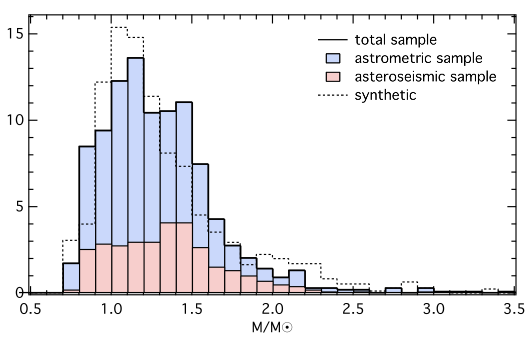
\includegraphics[height=0.36\textwidth]{pics/RG_distribution.png}
    }
    \subfloat[Белые карлики (класса DA)]{
        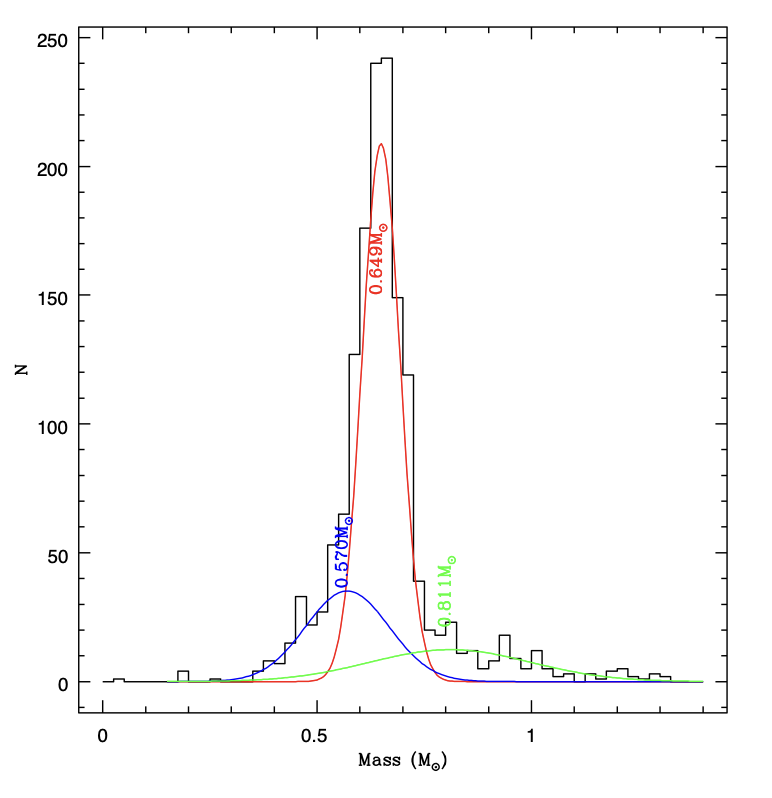
\includegraphics[height=0.4\textwidth]{pics/WD_distribution.png}
    }
    \caption{Распределения масс для красных гигантов и белых карликов, взятые из работ \cite{SDSS} и \cite{RedGiantMasses}. В случае белых карликов авторы также попытались представить распределение в виде суммы трёх гауссиан.}
    \label{fig:RG_WD_dists}
\end{figure}

Используя эти данные, можно численно оценить плотность априорного распределения для $m_\text{giant} / m_\text{dwarf}$. Но это трудоёмко и не гарантирует, что результат получится правильным, поскольку в тесных двойных системах эволюция может протекать по-другому, и распределение масс может отличаться от распределения среди звёзд в целом.

Может быть, правильное априорное распределение подобрать нельзя. Поэтому мы решили взять несколько вариантов и посмотреть, как меняется результат.

Мы остановились на следующих распределениях:
\begin{enumerate}
    \item $q \sim \operatorname{Uniform}(0.1, 10)$
    \item $q^{-1} \sim \operatorname{Uniform}(0.1, 10)$
    \item $q = \dfrac{m_\text{giant}}{m_\text{dwarf}}$, где: $
    \begin{cases}
        m_\text{giant} \sim \operatorname{Uniform}(0.6 M_\odot, 10 M_\odot) \\
        m_\text{dwarf} \sim \operatorname{Uniform}(0.3 M_\odot, 1.44 M_\odot)
    \end{cases}
    $
\end{enumerate}

В последнем распределении мы учли, что масса белого карлика должна быть меньше предела Чандрасекара, а масса красного гиганта должна быть больше $0.6 M_\odot$, чтобы он успел проэволюционировать за время существования Галактики.

На рис. \ref{pics/q_prior.pdf} изображена плотность вероятности для распределения (3).

\vspace{0.5em}

\fig{pics/q_prior.pdf}{
Один из вариантов априорного распределения для соотношения масс (если принять, что масса каждого из компонентов по отдельности имеет равномерное распределение). На двух графиках изображено одно распределение, но в разных масштабах.}

У равномерного априорного распределения есть преимущество перед остальными: при его использовании оценка параметров методом максимального правдоподобия (MAP) совпадает с оценкой методом максимальной апостериорной вероятности (MLE).

При репараметризации (например, замене $q$ на $q^{-1}$) функция правдоподобия преобразуется как обычное арифметическое выражение, и точка максимума преобразуется согласованно с заменой.

При этом апостериорная вероятность преобразуется как распределение: она умножается на новую априорную вероятность, у неё сохраняется интеграл, и максимум в старых переменных может отбросить неизвестно куда.

В качестве ответа в данной работе мы хотели бы получить величину $q = m_\text{giant} / m_\text{dwarf}$, а не, например, массы гиганта и карлика по отдельности. Поэтому в качестве основного варианта мы используем (1), где именно величина $q$ имеет равномерное априорное распределение.



\subsect{Исследованные модели}
\label{sect:Models}

Некоторые вещи в вероятностной модели можно выбирать по-разному. Во-первых, можно использовать разные атмосферные модели, что влияет на температурную зависимость спектральной плотности излучения и коэффициентов потемнения к краю. Во-вторых, можно по-разному выбирать априорные распределения, как описано в предыдущем разделе.

Мы решили рассмотреть несколько моделей и изучить, как меняются апостериорные оценки параметров и оптимальная кривая блеска.

В качестве главной мы выбрали модель с атмосферной моделью PHO\-E\-NIX и равномерным априорным распределением для соотношения масс $q$. В аннотации и заключении приведены именно её результаты.

Чтобы задать дополнительные модели, мы варьировали характеристики главной модели по одной за раз.
Так, мы рассмотрели одну дополнительную модель с чернотельной аппроксимацией спектра и две дополнительные модели с другими априорными распределениями для $q$.

В чернотельной модели аппроксимация распространяется только на спектр, но не на потемнение к краю. Потемнение к краю мы вычисляем с помощью коэффициентов Кларета, выведенных на основе всё той же модели PHOENIX.

% Мы рассмотрели следующие варианты:
% \begin{enumerate}
%     \item Модель с чернотельной аппроксимацией спектра. В этом случае мы использовали априорное распределение (1) для соотношения масс.
%     \item Модель с атмосферной моделью PHOENIX и априорным распределением (2) для соотношения масс.
%     \item Модель с атмосферной моделью PHOENIX и априорным распределением (3) для соотношения масс.
% \end{enumerate}

% Кроме того, мы рассмотрели модель с чернотельной аппроксимацией спектра

Результаты всех четырёх моделей и их сравнение приведены в следующей главе.










% В разделе \ref{sect:q_prior} мы показали, что есть неоднозначность при выборе априорного распределения для соотношения масс. Поэтому мы решили исследовать несколько вариантов и посмотреть, как это влияет на результат.






\sect{Результаты}

Мы получили апостериорное распределение вероятностей для параметров системы и насемплировали из него, как описано в разделе \ref{sect:Sampling}.

Количество семплов --- 30\,720, эффективный размер выборки (т.е. количество независимых семплов, которое давало бы ту же статистическую мощность) --- около 8\,500.

Каждому семплу соответствует кривая блеска. На их основе мы построили график с доверительным интервалом (рис. \ref{pics/ribbon.pdf}).

\fig[0.75]{pics/ribbon.pdf}{Насемплированные кривые блеска для главной модели. Изображен доверительный интервал $1\sigma$ для ожидаемых значений блеска при каждой фазе. Он более узкий, чем разброс точек, поскольку отражает накопленную статистику от всех измерений. Также изображены наблюдения блеска вместе с инструментальными погрешностями. Скорее всего, помимо инструментальных есть и другие источники ошибок, см. раздел \ref{sect:Brilliance}.}

Также мы построили апостериорные распределения каждого случайного параметра по отдельности:

\begin{figure}
\centering
\vspace{-1em}
\newcommand{\fourthwidth}{0.49\textwidth}
\subfloat{
    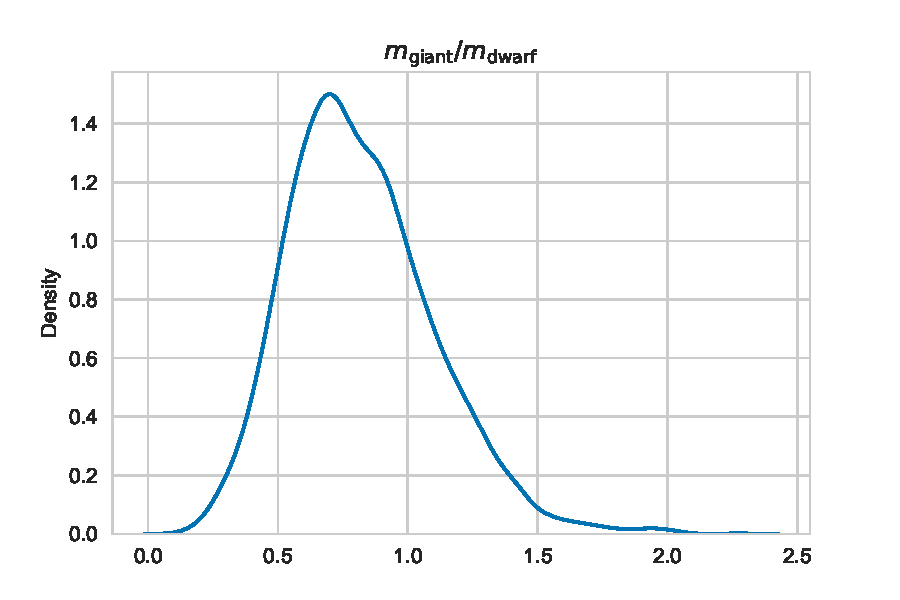
\includegraphics[width=\fourthwidth]{pics/mass_ratio.pdf}
}
\subfloat{
    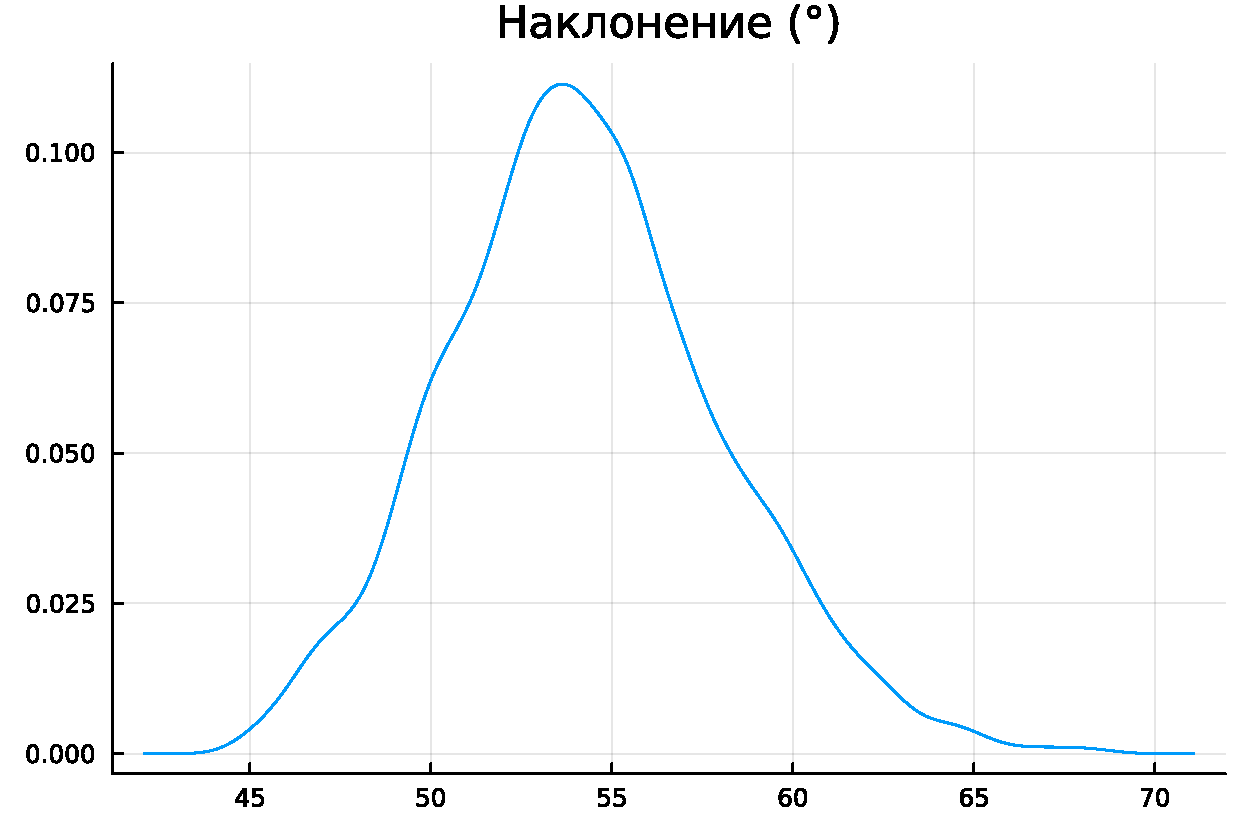
\includegraphics[width=\fourthwidth]{pics/inclination.pdf}
}\\[-0.5em]
\subfloat{
    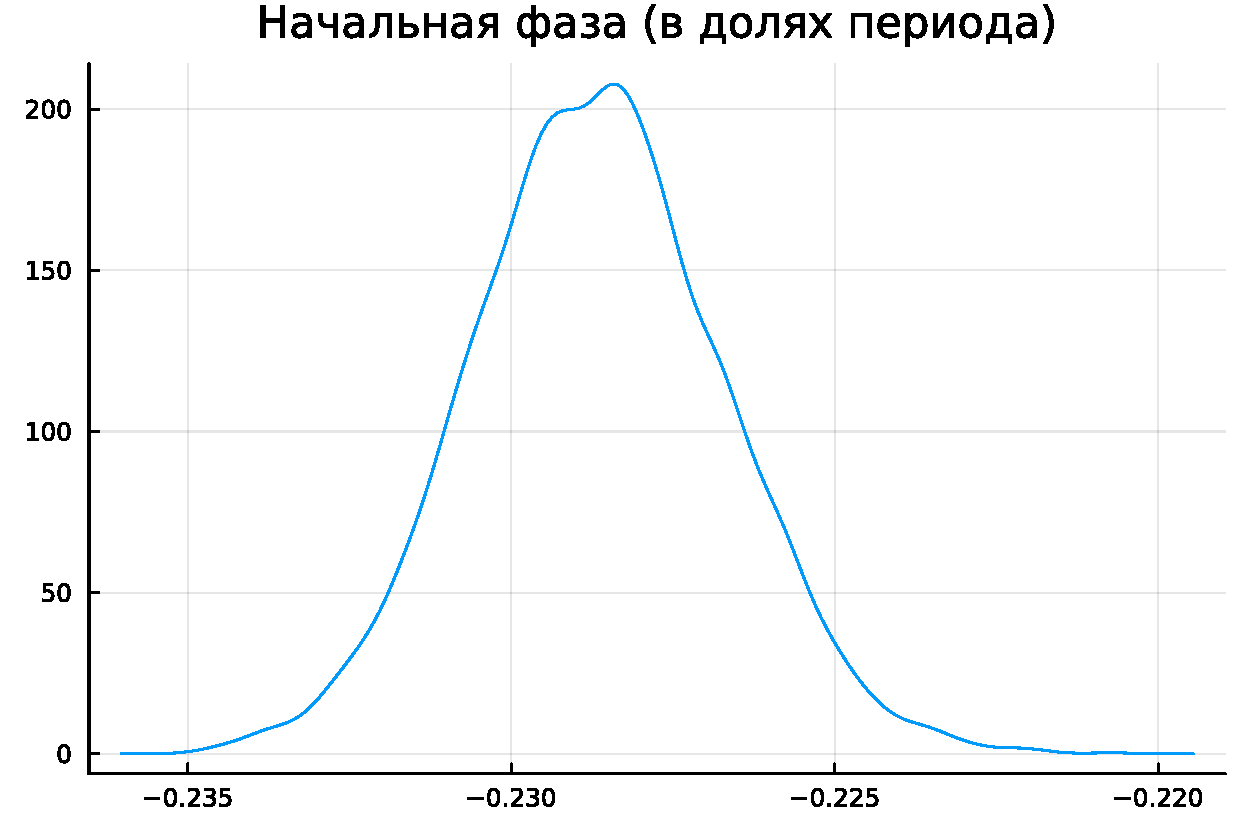
\includegraphics[width=\fourthwidth]{pics/initial_phase.pdf}
}
\subfloat{
    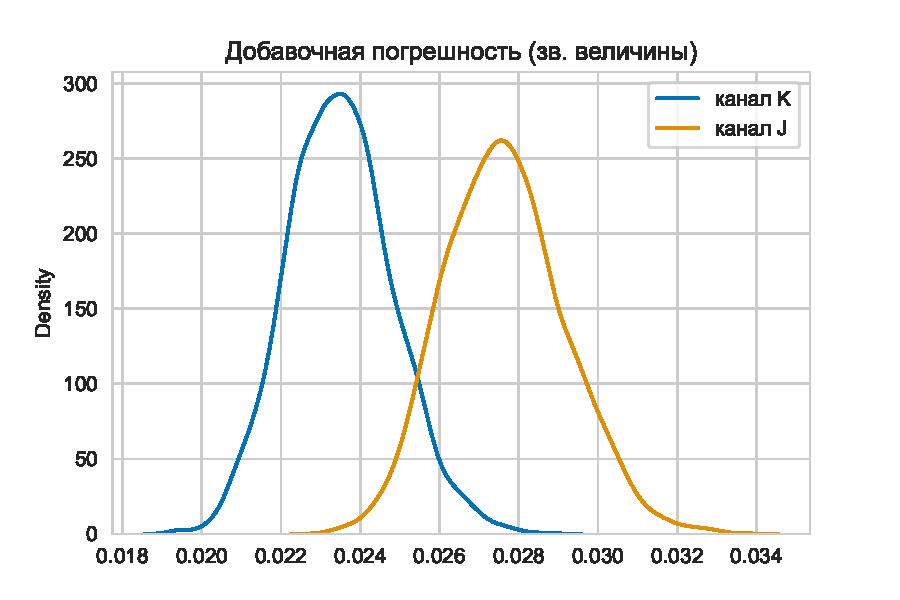
\includegraphics[width=\fourthwidth]{pics/sigma_common.pdf}
}
\label{fig:dists}
\caption{Апостериорные распределения параметров (главной) модели.}
\end{figure}


\subsect{Влияние модели излучения}

В предыдущих работах, в которых моделировались кривые блеска T Северной Короны \cite{Shanbaz,Belczynski,Tatarnikova,Maslennikova}, использовалось чернотельное приближение для спектра.

Мы же используем модель PHOENIX \cite{PHOENIX}, предназначенную для получения реалистичных спектров звёзд. Она учитывает линии поглощения и эмиссии, ненулевую оптическую толщину атмосферы и другие эффекты.

Чтобы определить, насколько это влияет на результат, мы запустили семплирование с обеими моделями и посмотрели, как меняется совместное распределение двух наиболее интересных параметров: соотношения масс и наклонения орбиты (рис. \ref{pics/biplot_different_L.pdf}).

\fig[0.9]{pics/biplot_different_L.pdf}{Совместное распределение соотношения масс ($q$) и наклонения орбиты ($i$) T Северной Короны при разных моделях излучения: чернотельной и PHOENIX. Значения генерировались из апостериорного распределения с учетом наблюдений блеска в каналах $J$ и $K$. В качестве априорного распределения для $q$ бралось равномерное. В закрашенные области попадает 68\%, в области, очерченные линиями --- 95\% сгенерированных значений (аналогично одномерным доверительным интервалам $\pm1\sigma$ и $\pm2\sigma$). Точками отмечены максимумы апостериорной вероятности.}

Видно, что смена модели излучения приводит к смещению по оси угла, а распределение по массам остаётся практически неизменным. Эффект от реалистичной модели атмосферы оказывается незначительным.

Также мы построили кривые блеска, соответствующие максимальному правдоподобию (рис. \ref{pics/mle_different_L.pdf}). Видно, что при разных моделях излучения они практически совпадают.

\fig[0.75]{pics/mle_different_L.pdf}{Кривые блеска, соответствующие параметрам с максимальным правдоподобием, для разных моделей излучения ($m_\text{giant} / m_\text{dwarf} = 0.68$, $i = 55.5^\circ$ для модели PHOENIX, $m_\text{giant} / m_\text{dwarf} = 0.64$, $i = 55.7^\circ$ для модели с чернотельным спектром).}


\subsect{Влияние априорных распределений}

Для двух наиболее интересных параметров (соотношения масс и наклонения) мы построили совместное распределение (рис. \ref{pics/biplot_different_q.pdf}).

Видно, что отношение масс и наклонение орбиты сильно скоррелированы. Это связано с тем, что чем больше масса карлика, тем сильнее деформирован красный гигант и тем больше амплитуда колебаний яркости. Но это можно скомпенсировать уменьшением наклона орбиты.

В разделе \ref{sect:q_prior} мы обсуждали, что априорное распределение для соотношения масс можно выбирать по-разному. Это приводит к смещению итогового распределения, что также отражено на рис. \ref{pics/biplot_different_q.pdf}.

Смещение вызвано тем, что разные априорные распределения заставляют модель предпочитать решения с большим или меньшим $q$ (рис \ref{pics/q_prior.pdf}).

\fig[0.9]{pics/different_priors.pdf}{Плотность вероятности различных вариантов априорного распределения соотношения масс, которые мы использовали.}

\fig[0.9]{pics/biplot_different_q.pdf}{Совместное распределение соотношения масс ($q$) и наклонения орбиты ($i$) T Северной Короны при разных априорных распределениях для $q$. Значения генерировались из апостериорного распределения с учетом наблюдений блеска в каналах $J$ и $K$. В закрашенные области попадает 68\% сгенерированных значений (аналогично одномерному доверительному интервалу $\pm1\sigma$). Точками отмечены максимумы апостериорной вероятности для $q$ и $i$. Затенена область, запрещённая пределом Чандрасекара и известной лучевой скоростью красного гиганта (см. раздел \ref{sect:Chandrasekhar}).}

% Также мы построили кривые блеска, соответствующие точкам максимальной апостериорной вероятности (рис. \ref{pics/map_different_q.pdf}). Видно, что хоть параметры и различаются, оптимальные кривые блеска для разных априорных распределений практически совпадают.

Это означает, что есть вырождение: кривая блеска определяется не соотношением масс $q$ и наклонением $i$ по отдельности, а некоторой функцией $f(q,i)$. Поэтому мы плохо различаем разные пары $(q,i)$ с одинаковым значением $f$.

Устранить неоднозначность можно, только добавляя в анализ другие измерения вдобавок к наблюдениям блеска.


% \fig[0.75]{pics/map_different_q.pdf}{Кривые блеска T Северной Короны, соответствующие параметрам с максимальной апостериорной вероятностью (для разных априорных распределений соотношения масс).}


\subsect{Сравнение с другими работами}

Простейший способ определить соотношение масс --- это измерить отношение лучевых скоростей:
\[
\frac{m_\text{giant}}{m_\text{dwarf}} = \frac{K_\text{dwarf}}{K_\text{giant}}
\]

Именно так поступили в работах \cite{Kraft, H_alpha}. Результаты приведены в таблице \ref{tab:comparison}.

Из лучевых скоростей, однако, нельзя напрямую определить наклонение. Но в работе \cite{H_alpha} удалось сильно ограничить возможные наклонения при данном соотношении масс, исходя из отсутствия затмений ($i < 70^\circ$) и предела Чандрасекара ($i > 65^\circ$).


\begin{table}[h]
\caption{\centering Сравнение работ разных авторов}
\label{tab:comparison}
\SetTblrInner{rowsep=0.4em}
\centering
\begin{tblr}{|Q[c,m] | Q[c,m] | X[c,m] | X[l,m]|}
\hline
$\dfrac{m_\text{giant}}{m_\text{dwarf}}$ & Наклонение & Источник & Данные \\
\hline
1.4 & -- & \citeauthor{Kraft} (\citeyear{Kraft}) \cite{Kraft} & Лучевые скорости \\
\hline
1/3 & $\brk!{40^{+6}_{-2}}\, {}^\circ$ & Shanbaz et al. (\citeyear{Shanbaz}) \cite{Shanbaz} & Кривые блеска в инфракрасном диапазоне ($J$) \\
\hline
$0.6 \pm 0.2$ & $60^\circ \pm 5^\circ$ &\citeauthor{Belczynski} (\citeyear{Belczynski}) \cite{Belczynski} & Кривые блеска в инфракрасном и видимом диапазоне ($V$ \& $J$) \\
\hline
$0.82 \pm 0.10$ & $67^\circ \pm 3^\circ$ & Stanishev et al. (\citeyear{H_alpha}) \cite{H_alpha} & Лучевые скорости, отсутствие затмений \\
\hline
$0.65 \pm 0.15$ & $57^\circ \pm 5^\circ$ & \citeauthor{Tatarnikova} (\citeyear{Tatarnikova}) \cite{Tatarnikova} & Кривые блеска в инфракрасном диапазоне ($J$) \\
\hline
$0.57^{+0.20}_{-0.07}$ & $\brk!{58^{+5}_{-3}}\, {}^\circ$ & Maslennikova et al. (\citeyear{Maslennikova}) \cite{Maslennikova} & Кривые блеска в инфракрасном диапазоне ($J$ \& $K$) \\
\hline
$\resultq$ & $\resulti$ & Настоящая работа (2024) & Кривые блеска в инфракрасном диапазоне ($J$ \& $K$) \\
\hline
\end{tblr}
\end{table}

В работах \cite{Tatarnikova, Maslennikova} на одном графике строились возможные наклонения и соотношения масс T Северной Короны (рис. \ref{pics/Maslennikova.png}, \ref{pics/Tatarnikova.png}). Их результаты в целом согласуются с нашим рис. \ref{pics/biplot_different_q.pdf}.


\fig[0.55]{pics/Maslennikova.png}{Возможные наклонения и соотношения масс компонентов T Северной Короны, полученные в работе \cite{Maslennikova}. Кривые очерчивают ограничения, соответствующие $m_\text{dwarf} < 1.44 M_\odot$, $m_\text{giant} > 0.6 M_\odot$ и отсутствию затмений. В серую область, по утверждению авторов статьи, по критерию Фишера попадает 90\% моделей, описывающих наблюдаемые данные. Крестом обозначены параметры, соответствующие наименьшему отклонению от наблюдений ($i = 58^\circ$, $q = 0.57$)}

\fig[0.3]{pics/Tatarnikova.png}{Наклонения и соотношения масс компонентов T Северной Короны, полученные в работе \cite{Tatarnikova}. Темно-серая область соответствует доверительному интервалу 75\%, светло-серая --- 90\%. В работе использовался критерий Фишера. Сплошная линия соответствует $m_\text{giant} = 0.6 M_\odot$, пунктирная линия --- отсутствию затмений, линия из точек --- $m_\text{dwarf} = 1.44 M_\odot$.}

Результаты в целом схожи. Например, практически все работы, включая нашу, показывают, что гигант легче карлика.


\subsect{Runs Test}\label{sect:RunsTest}

Как видно из рис. \ref{pics/mle_different_L.pdf}, наилучшая модельная кривая плохо описывает данные в окрестности главного минимума.

Чтобы более тщательно исследовать этот вопрос, мы построили разность между экспериментальными и модельными значениями звездной величины (рис. \ref{pics/residuals.pdf}). Видно, что невязка не однородна по времени. Есть участки, где она преимущественно положительная.

\fig[0.75]{pics/residuals.pdf}{Разность между экспериментальными и модельными значениями звездной величины. Использовался метод максимального правдоподобия. Цветом обозначен знак разности.}

Мы применили runs test (критерий Вальда-Вольфовица). Это статистический тест, который опирается на последовательность знаков невязок. Он проверяет нулевую гипотезу о том, что невязки независимы и одинаково распределены. В отличие от, например, критерия $\chi^2$, runs test не требует знания погрешностей, которые мы не можем оценить напрямую.

% Он удобен для нашего случая, поскольку не требует знания погрешностей, которые мы не можем оценить напрямую.

Runs test показал, что p-value < $10^{-14}$. Это означает, что наша модель эллипсоидальной переменности неверна. Иначе точки были бы симметрично распределены относительно предсказанной кривой.

Похожая проблема была в других работах. Например, в \cite{Shanbaz}, чтобы объяснить главный минимум, предлагается добавить в модель неподвижное тёмное пятно на «носике» красного гиганта. Тёмное пятно должно иметь радиус порядка $20^\circ$ и иметь температуру на 750 ${}^\circ$К ниже, чем предсказывает формула гравитационного потемнения.


\structel{ЗАКЛЮЧЕНИЕ}

% В данной работе мы построили модель кривых блеска T Северной Короны, используя метод Монте-Карло. Мы нашли апостериорное распределение параметров системы и на его основе насемплировали кривые блеска.

% Мы сравнили результаты с другими работами и обнаружили, что они в целом согласуются.

% Мы обнаружили, что наша модель не описывает данные в окрестности более глубокого минимума. Это может быть связано с тем, что мы не учли некоторые физические процессы, такие как магнитные поля, конвекция и др.

% Мы также обнаружили, что невязки не являются независимыми и однородно распределёнными. Это говорит о том, что наша модель эллипсоидальной переменности неверна.

% В дальнейшем планируется улучшить модель, учтя дополнительные физические процессы, и провести более тщательный анализ невязок.

Мы построили компьютерную модель переменных звёзд, относящихся к эллипсоидальному типу. Она позволяет строить синтетические кривые блеска в инфракрасном диапазоне. Мы учли приливную деформацию звезды и эффект гравитационного потемнения; использовали модель звёздной атмосферы PHOENIX для получения спектров и учета потемнения к краю.

Мы проанализировали экспериментальные кривые блеска симбиотической двойной звезды T Северной Короны в спектральных каналах $J$ и $K$, охватывающие 1996--2003 и 2008--2021 годы. С помощью байесовского подхода и библиотеки вероятностного программирования Turing.jl мы получили апостериорное распределение вероятностей для параметров системы, главные из которых --- наклонение орбиты и соотношение масс звёзд-компаньонов.

Мы получили, что соотношение масс компонентов $m_\text{giant} / m_\text{dwarf} = \resultq$, а наклонение орбиты $i = \resulti$ (наиболее вероятные значения с доверительным интервалом 68\%).

Мы показали, что эти оценки смещаются в зависимости от выбора априорного распределения для соотношения масс. Это означает, что данные о блеске недостаточно ограничивают апостериорное распределение.

Наши оценки соотношения масс и наклонения в целом согласуются с другими работами (таблица \ref{tab:comparison}). Например, большинство других работ также предсказывает $m_\text{giant} < m_\text{dwarf}$.

Традиционно для моделирования кривых блеска в инфракрасном диапазоне используется модель абсолютно черного тела. Мы использовали атмосферную модель PHOENIX, показали, что это влияет на оценку наклонения, но не соотношения масс, и что эффект слабый. Следовательно, на практике можно использовать простую чернотельную модель.

Мы применили критерий Вальда-Вольфовица (runs test) и обнаружили, что наилучшая модельная кривая блеска с высокой статистической значимостью расходится с наблюдениями в окрестности более глубокого минимума. Это говорит о том, что модель эллипсоидальной переменности не вполне применима к T Северной Короны.


\showbib

\end{document}
